% Brian Mc George - MCGBRI004
% Jacques Heunis - HNSJAC003
% Timothy Gwynn - GWNTIM001
% Due: 31-07-2015
% Stage One - Software Engineering  - CSC3003S
\documentclass[a4paper,10pt]{article}
%**************************************************************************************************
% PACKAGES
%**************************************************************************************************
\usepackage{amsmath, amsthm, amsfonts, amssymb}
\usepackage{graphicx,color}
\usepackage{bm}	
\usepackage{float}
\usepackage{caption, subcaption}
%\usepackage{vector}

%**************************************************************************************************
% DEFAULT SETTINGS
%**************************************************************************************************
\marginparwidth -20 true pt    % Width of marginal notes.
\oddsidemargin  -10 true pt       % Note that \oddsidemargin=\evensidemargin
\evensidemargin -10 true pt
\topmargin -0.5 true in        % Nominal distance from top of page to top of
\textheight 9.75 true in         % Height of text (including footnotes and figures)
\textwidth 7 true in        % Width of text line.
\parindent=10pt                  % Do not indent paragraphs
\parskip= 1 ex
\columnseprule = 0.1pt
\footskip = 30 true pt
\hoffset = -0.1 true in
\voffset = -0.1 true in
\abovedisplayskip 1 true pt
\abovedisplayshortskip 1 true pt
\topsep 0 true pt
\newcommand*\varhrulefill[1][0.4pt]{\leavevmode\leaders\hrule height#1\hfill\kern0pt}

%**************************************************************************************************
% DOCUMENT DETAILS
%**************************************************************************************************


%**************************************************************************************************
% MAIN DOCUMENT 
%**************************************************************************************************

\begin{document}
\begin{titlepage} \begin{center} 
		\textsc{\LARGE University of Cape Town}
		\\[1.5cm] \textsc{\Large Software Engineering Stage Two\\CSC3003S}
		\\[0.5cm]
		\noindent\rule[0.4mm]{\textwidth}{0.1mm}
		\\[0.4cm] { \huge \bfseries Tempest Trace \\[0.4cm] }
		\noindent\rule[0.4mm]{\textwidth}{0.1mm}
		\\[1cm]
		\begin{minipage}[t]{0.4\textwidth}
		\begin{flushleft}\large \emph{Authors:}\\ Brian Mc George - MCGBRI004 \\ Jacques Heunis - HNSJAC003 \\ Timothy Gwynn - GWYTIM001\end{flushleft}
		 \end{minipage} \begin{minipage}[t]{0.4\textwidth} 
		\begin{flushright} \large \emph{Supervisor:} \\ Assoc. Prof.~Patrick Marais\\patrick@cs.uct.ac.za\end{flushright}
		\begin{flushright} \large \emph{Tutor:} \\ Codie Roelf\\Codie.Roelf@alumni.uct.ac.za\end{flushright}
		 \end{minipage} \vfill {\large \today}
		\end{center}
		\end{titlepage}
\newpage
\tableofcontents
\newpage

\section{Use Case Narratives}
\subsection{Move player}
\textbf{Actor:} Player\smallskip\\
The player specifies which direction he/she wants the character to move in. The system performs collision detection to detect whether the input movement is allowed. If the movement is allowed the player's character is appropriately displaced in the system and the appropriate animation is played. The system represents this graphically for both players. The system checks whether the player has reached the end goal and if so ends the game.\smallskip\\
If the movement is not allowed the player's character will not move and no adjustments will be made to the system.

\subsection{Jump player}
\textbf{Actor:} Player\smallskip\\
The player specifies he/she wants the character to jump. The system performs collision detection to detect whether the input movement is allowed. If the movement is allowed the player's character is appropriately displaced in the system depending on what sort of obstacle is in close proximity and in front of the player and the appropriate animation is played. If there is a box/low wall in front of the player character it will vault over it. If there is a taller wall the player character will grab the top of the wall and pull itself up. If the wall is too tall the player will just perform the standard jump. If there is no obstacle the player will perform a standard jump. The system represents this graphically for both players and outputs appropriate sound effects. The system checks whether the player has reached the end goal and if so ends the game.\smallskip\\
If the movement is not allowed the player's character will not move and no adjustments will be made to the system.

\subsection{Slide player}
\textbf{Actor:} Player\smallskip\\
The player specifies he/she wants the character to slide. The system performs collision detection to detect whether the input movement is allowed. If the movement is allowed the player's character is appropriately displaced in the system depending on what slope is in front of the player and the appropriate animation is played. The system represents this graphically for both players and outputs appropriate sound effects. The system checks whether the player has reached the end goal and if so ends the game.\smallskip\\
If the movement is not allowed the player's character will not move and no adjustments will be made to the system.

\subsection{Respawn player}
\textbf{Actor:} Player\smallskip\\
The player's character dies. The system checks where the closest respawn point behind the player is. If there are no obstacles at the spawn location, the player's character appears at the location and the appropriate animation is played. The system represents this graphically for both players and updates the player's character's location.  The system is updated to reflect the player's new position.\smallskip\\
If the spawn location is blocked, perhaps by the other player or an AI unit the game will delay the respawn up to 1.5 seconds until the spawn location is cleared otherwise it will pick the next closest spawn location.

\subsection{Use smoke grenade}
\textbf{Actor:} Player\smallskip\\
The player specifies he/she wants the character to use a smoke bomb. The system checks whether the player has smoke grenades playing. If the player has smoke grenades available the appropriate animation is displayed along with the appropriate sound effect and a new smoke cloud object is created at the player's location. Over time the smoke cloud object will shrink and eventually be removed.\smallskip\\
If the player has no smoke grenade an error sound will be played.

\subsection{Update mobile AI behaviour}
\textbf{Actor:} Time\smallskip\\
Every 2 seconds the mobile AI updates its behaviour. The AI checks with the system whether it has a target, if it has a target it then checks whether that target is in line of sight, if the target is in line of sight then the AI moves towards the target. If the target is within sufficiently small distance and moving sufficiently slowly the AI will then shoot towards the target.\smallskip\\
If the target is not in line of sight the AI checks whether the other possible target is in line of sight, if this is the case it will switch targets, otherwise it will proceed to it's current target's last seen position. If it cannot find the player at the last seen position it will timeout and return back to patrolling. \smallskip\\
If the AI has no target it will attempt to acquire one by checking if there are any player characters in line of sight and sufficiently close, if there are none it will continue to patrol between predefined points.

\subsection{Update static AI behaviour}
\textbf{Actor:} Time\smallskip\\
Every 2 seconds the static AI updates its behaviour. The AI checks with the system whether it has a target, if it has a target, it then checks whether that target is in line of sight. If the target is in line of sight, then the AI increases its accuracy rating. The AI will then shoot towards the target.\smallskip\\
If the target is not in line of sight the AI checks whether the other possible target is in line of sight, if this is the case it will switch targets and reset its accuracy rating to a default. The AI will then shoot towards the target. If neither target is in line of sight the AI will remain in a passive state with a default accuracy rating until a valid target enters its line of sight at which point it will acquire the target.

\section{Analysis Class Model}
\begin{figure}[H]
	\begin{center}
		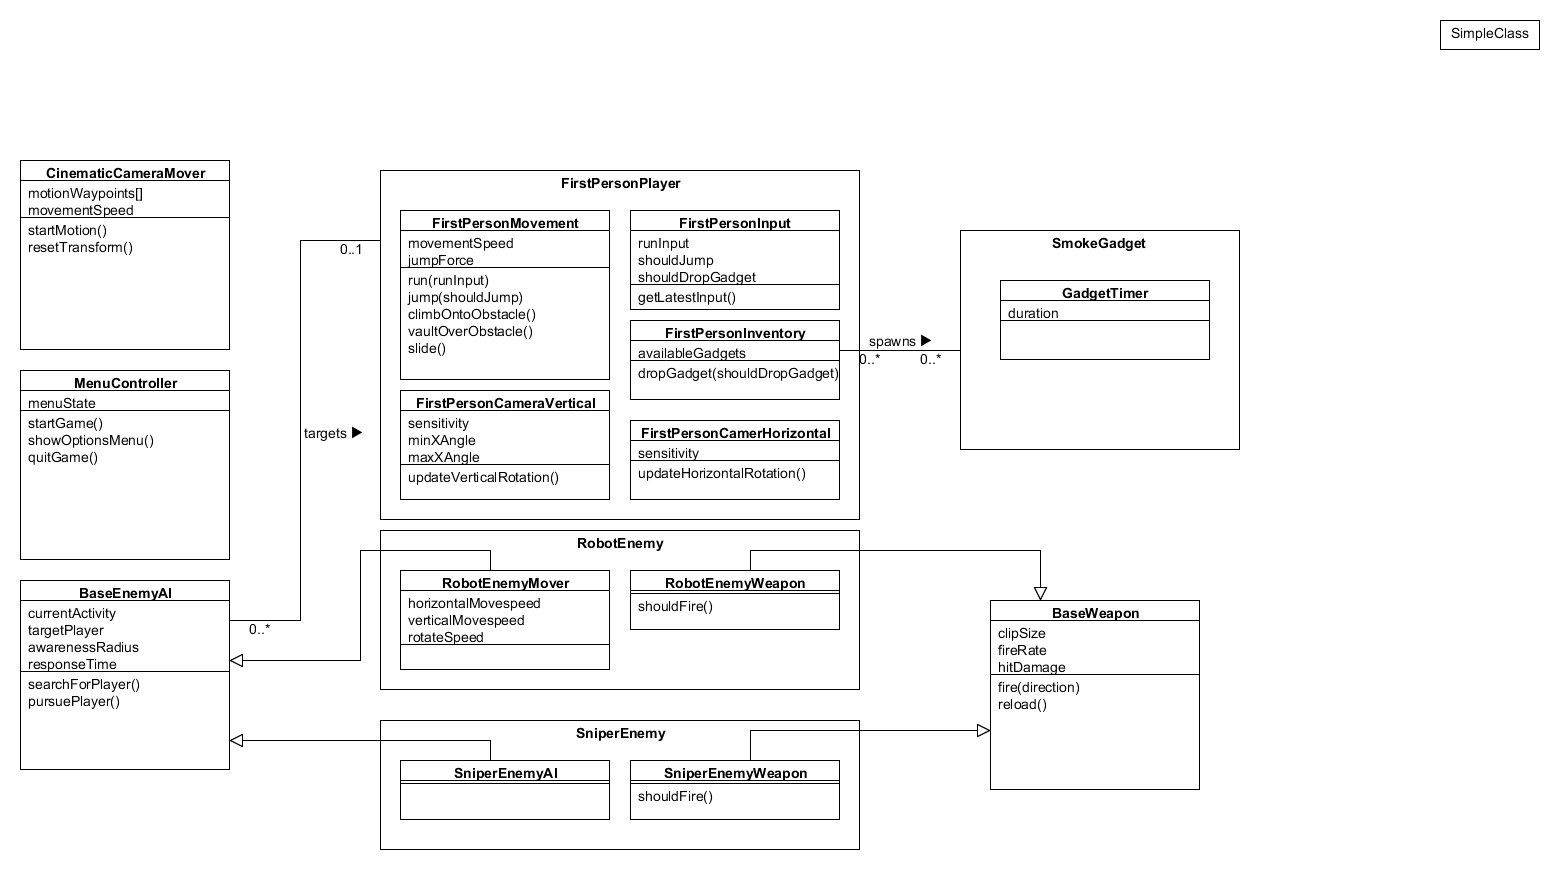
\includegraphics[scale=0.4]{images/AnalysisClassDiagram.png}
		\caption{An analysis class model for the predicted class/object requirements}
	\end{center}
\end{figure}
Here we show the classes that we predict will need to be implemented. In the above diagram FirstPersonPlayer, RobotEnemy, and SniperEnemy are used to indicate GameObjects or Prefabs in Unity, where the outer box (e.g RobotEnemy) represents a GameObject, and the classes within (RobotEnemyMover and RobotEnemyWeapon) are components attached to that object. \\
This is done so that the organisation and interaction of the scripts can be better communicated in a sense that closely matches the implementation. It has only been done for the more complex objects (for example CinematicCameraMover is likely to be the only script attached to the object) so as to preserve readability.

\section{State Diagrams}
\begin{figure}[H]
	\begin{center}
		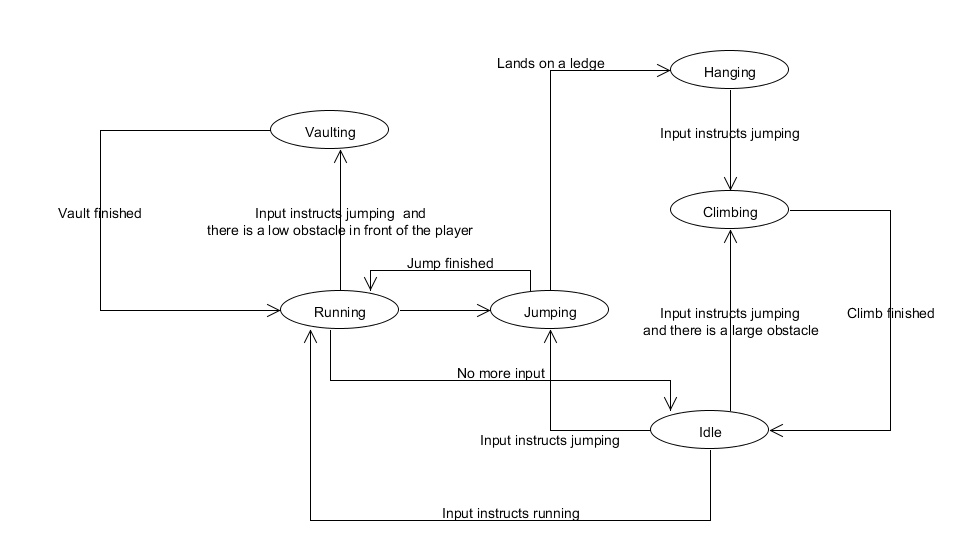
\includegraphics[scale=0.5]{images/PlayerStateMachine.png}
		\caption{A state machine for the player}
	\end{center}
\end{figure}
\begin{figure}[H]
	\begin{center}
		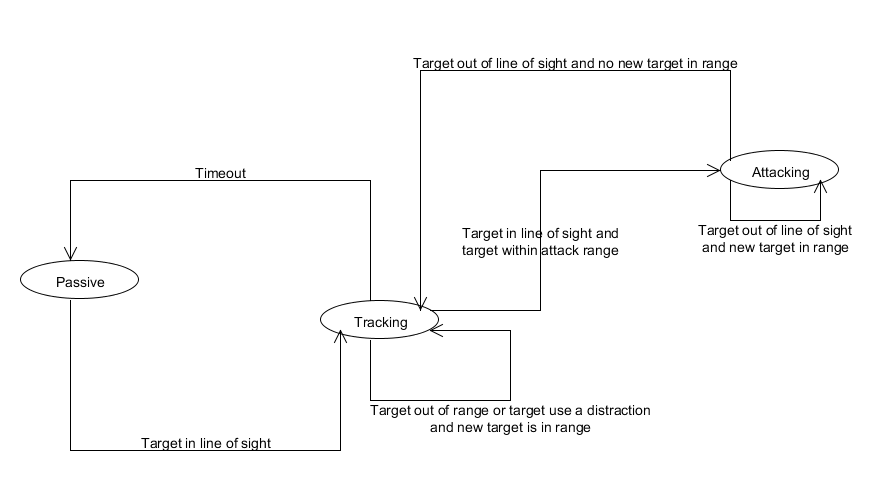
\includegraphics[scale=0.5]{images/EnemyStateMachine.png}
		\caption{A state machine for the 2 types of enemies in the game}
	\end{center}
\end{figure}

\section{Project Plan}
Refer to \textit{TempestTraceGanttChart.pdf}
\section{Test Plan}
    \subsection{Game ends when player reaches finish line}
        \textbf{Pre-conditions}\\
        Both players have not passed the finish line. 
        \smallskip\\\textbf{Input}\\
        A player passes the finish line.
        \smallskip\\\textbf{Expected output}\\
        The game timer stops and the end game screen is shown.
        
    \subsection{Player jumps forward}
        \textbf{Pre-conditions}\\
        Player is moving and no obstacle within half a metre in front of player. 
        \smallskip\\\textbf{Input}\\
        A player presses the jump button.
        \smallskip\\\textbf{Expected output}\\
        The player jump animation plays and the player moves both forward and upwards. 
        
    \subsection{Player climbs up ledge}
    \textbf{Pre-conditions}\\
    Obstacle is within half a metre in front of player and its height within a range of 1.5 metres to 2 metres. 
    \smallskip\\\textbf{Input}\\
    A player presses the jump button.
    \smallskip\\\textbf{Expected output}\\
    The player climb animation plays and the player moves upwards onto the obstacle.
    
    \subsection{Player vaults over obstacle}
    \textbf{Pre-conditions}\\
    Player is moving. Obstacle is within half a metre in front of player and its height is less than 1.5 metres. 
    \smallskip\\\textbf{Input}\\
    A player presses the jump button.
    \smallskip\\\textbf{Expected output}\\
    The player vault animation plays and the player moves onto the top of the obstacle.
    
    \subsection{Player cannot climb over high wall}
    \textbf{Pre-conditions}\\
    Player is moving. Obstacle is within half a metre in front of player and its height is more than 2 metres. 
    \smallskip\\\textbf{Input}\\
    A player presses the jump button.
    \smallskip\\\textbf{Expected output}\\
    The player jump animation plays and the player jumps forward but does not climb over wall.
        
    \subsection{Smoke bomb deployed}
    \textbf{Pre-conditions}\\
    Player has smoke bombs remaining.
    \smallskip\\\textbf{Input}\\
    A player presses the smoke bomb button.
    \smallskip\\\textbf{Expected output}\\
    The player smoke bomb throw animations plays and the bomb is thrown to the ground. When the bomb reaches the ground, a small explosion occurs and a smoke cloud covers the area.
    
    \subsection{Sniper fires at player}
    \textbf{Pre-conditions}\\
    Player is tracked by sniper.
    \smallskip\\\textbf{Input}\\
    No input from player.
    \smallskip\\\textbf{Expected output}\\
    The player is fire at by the sniper after two seconds.
    
    \subsection{Drone tracks player}
    \textbf{Pre-conditions}\\
    Player within line of sight of drone. Player within 50 metres from drone. Drone is not tracking a player already.
    \smallskip\\\textbf{Input}\\
    Player stays in vision of drone for at least one second.
    \smallskip\\\textbf{Expected output}\\
    The drone tries to get within range to fire at player. The drone fires at the player when within range.
    
    \subsection{Drone attacks player}
    \textbf{Pre-conditions}\\
    Player tracked by drone. Drone within attack range.
    \smallskip\\\textbf{Input}\\
    Player stays in vision of drone.
    \smallskip\\\textbf{Expected output}\\
    The drone fires at the player.    
    
    \subsection{Music changes when tracked by AI}
    \textbf{Pre-conditions}\\
    Not currently tracked by AI.
    \smallskip\\\textbf{Input}\\
    Player moves into vision of AI.
    \smallskip\\\textbf{Expected output}\\
    The player gets tracked by AI. Once tracked, the music transitions over three seconds to the intense music.
    
    \subsection{Music changes when no longer tracked by AI}
    \textbf{Pre-conditions}\\
    Currently tracked by AI.
    \smallskip\\\textbf{Input}\\
    Player stays out of sight of AI.
    \smallskip\\\textbf{Expected output}\\
    The drone state times out and transitions to passive state. Music transitions over three seconds to calm invigorating music.
        
\end{document}
